L'introduction est une section requise dans un rapport technique. Introduisez votre travail, l'idée de départ et les objectifs attendus. Un lecteur qui découvrirait votre projet au travers de cette introduction devrait ainsi être capable d'en comprendre le cadre, l'idée générale et les aboutissants du projet.

Le but de ce projet de bachelor consiste, premièrement, d'apporter plus de sécurité au système de pinces optiques par laser afin de faciliter son utilisation au quotidien. Deuxièmement, une proposition d'expérience avec un mode d'emploi compact est proposé pour le cours de NANO pour les systèmes industriels.Troisièmement, des tests de déplacements de microbilles dans différents milieux, de différentes viscosités, dans différents types de réservoirs ainsi que de multiples canaux.
\newpage
\section{Contexte}

Le kit de pinces optiques portables, Portable Optical Tweezers, est un dispositif qui permet de déplacer de microobjets grâce à un faisceau laser focalisé. L'entreprise qui fabrique ce kit, Thorlabs, est une entreprise américaine qui conçoit des composants optiques, des lasers, des instruments de mesure.

L'image ci-dessous (voir Figure \ref{chemin_laser_caméra}) montre le trajet parcouru par le laser (\textcolor{red}{en rouge}), ainsi que du microscope vers la caméra (\textcolor[RGB]{0, 120, 0}{en vert}).

\begin{figure}[H]
    \begin{center}
        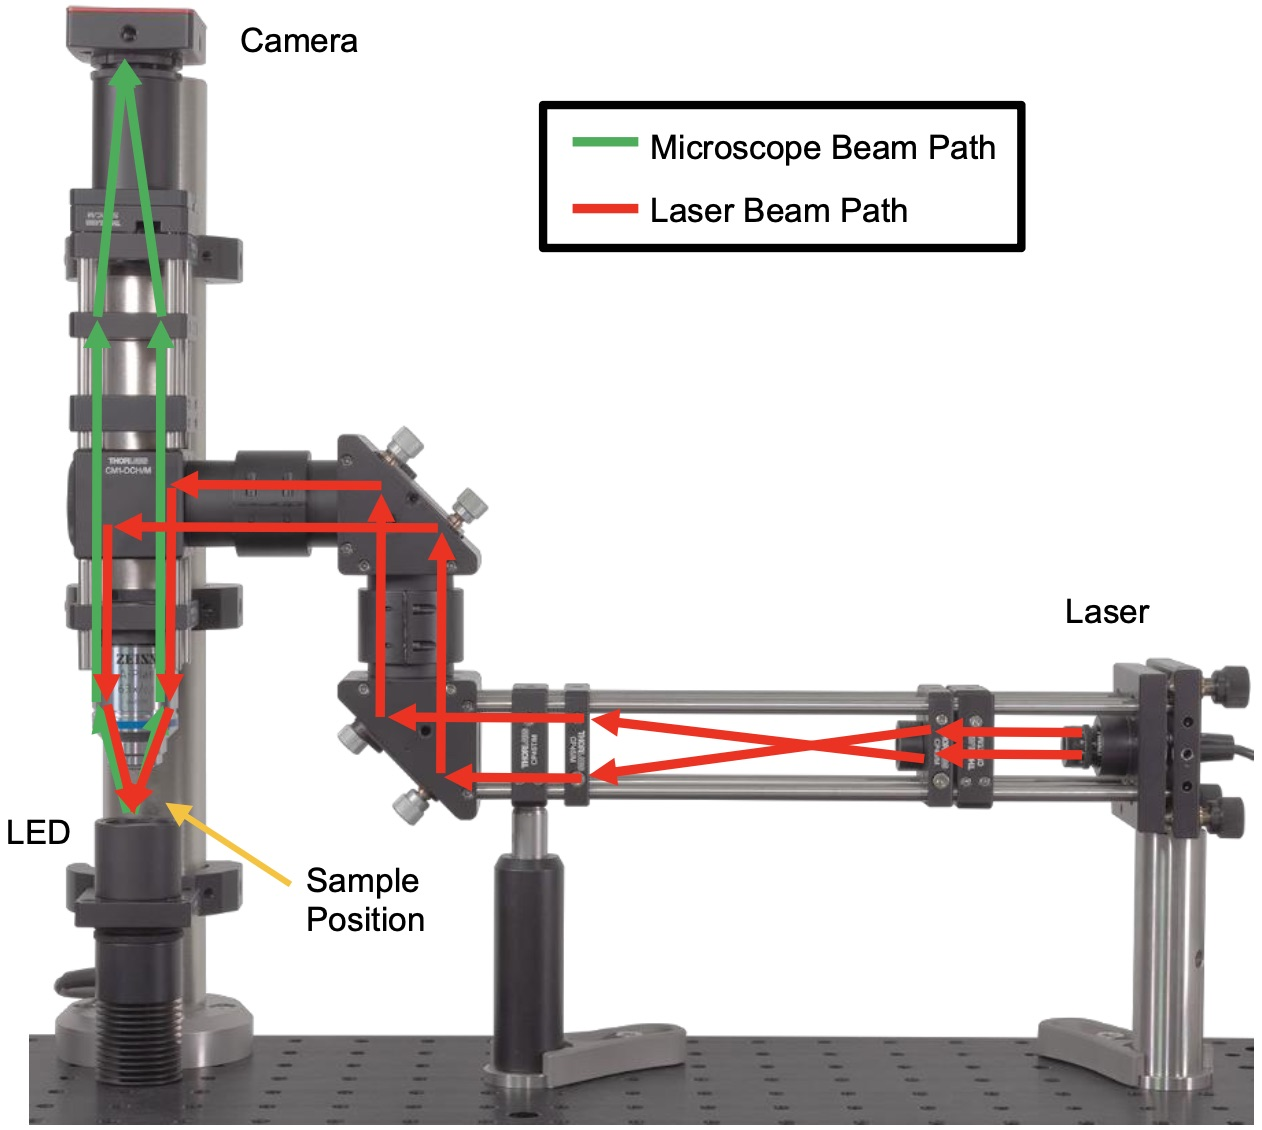
\includegraphics[width=0.7\textwidth]{assets/figures/Introduction/chemin_laser_camera.jpeg}
    \end{center}
    \caption{Trajet du laser et du microscope}
    \label{chemin_laser_caméra}
\end{figure}

La figure ci-dessous (voir Figure \ref{kit_vierge}) correspond au kit reçu lors du premier jour de TB. Le kit a été monté par un assistant du laboratoire COMATEC-LANS.

\begin{figure}[H]
    \begin{center}
        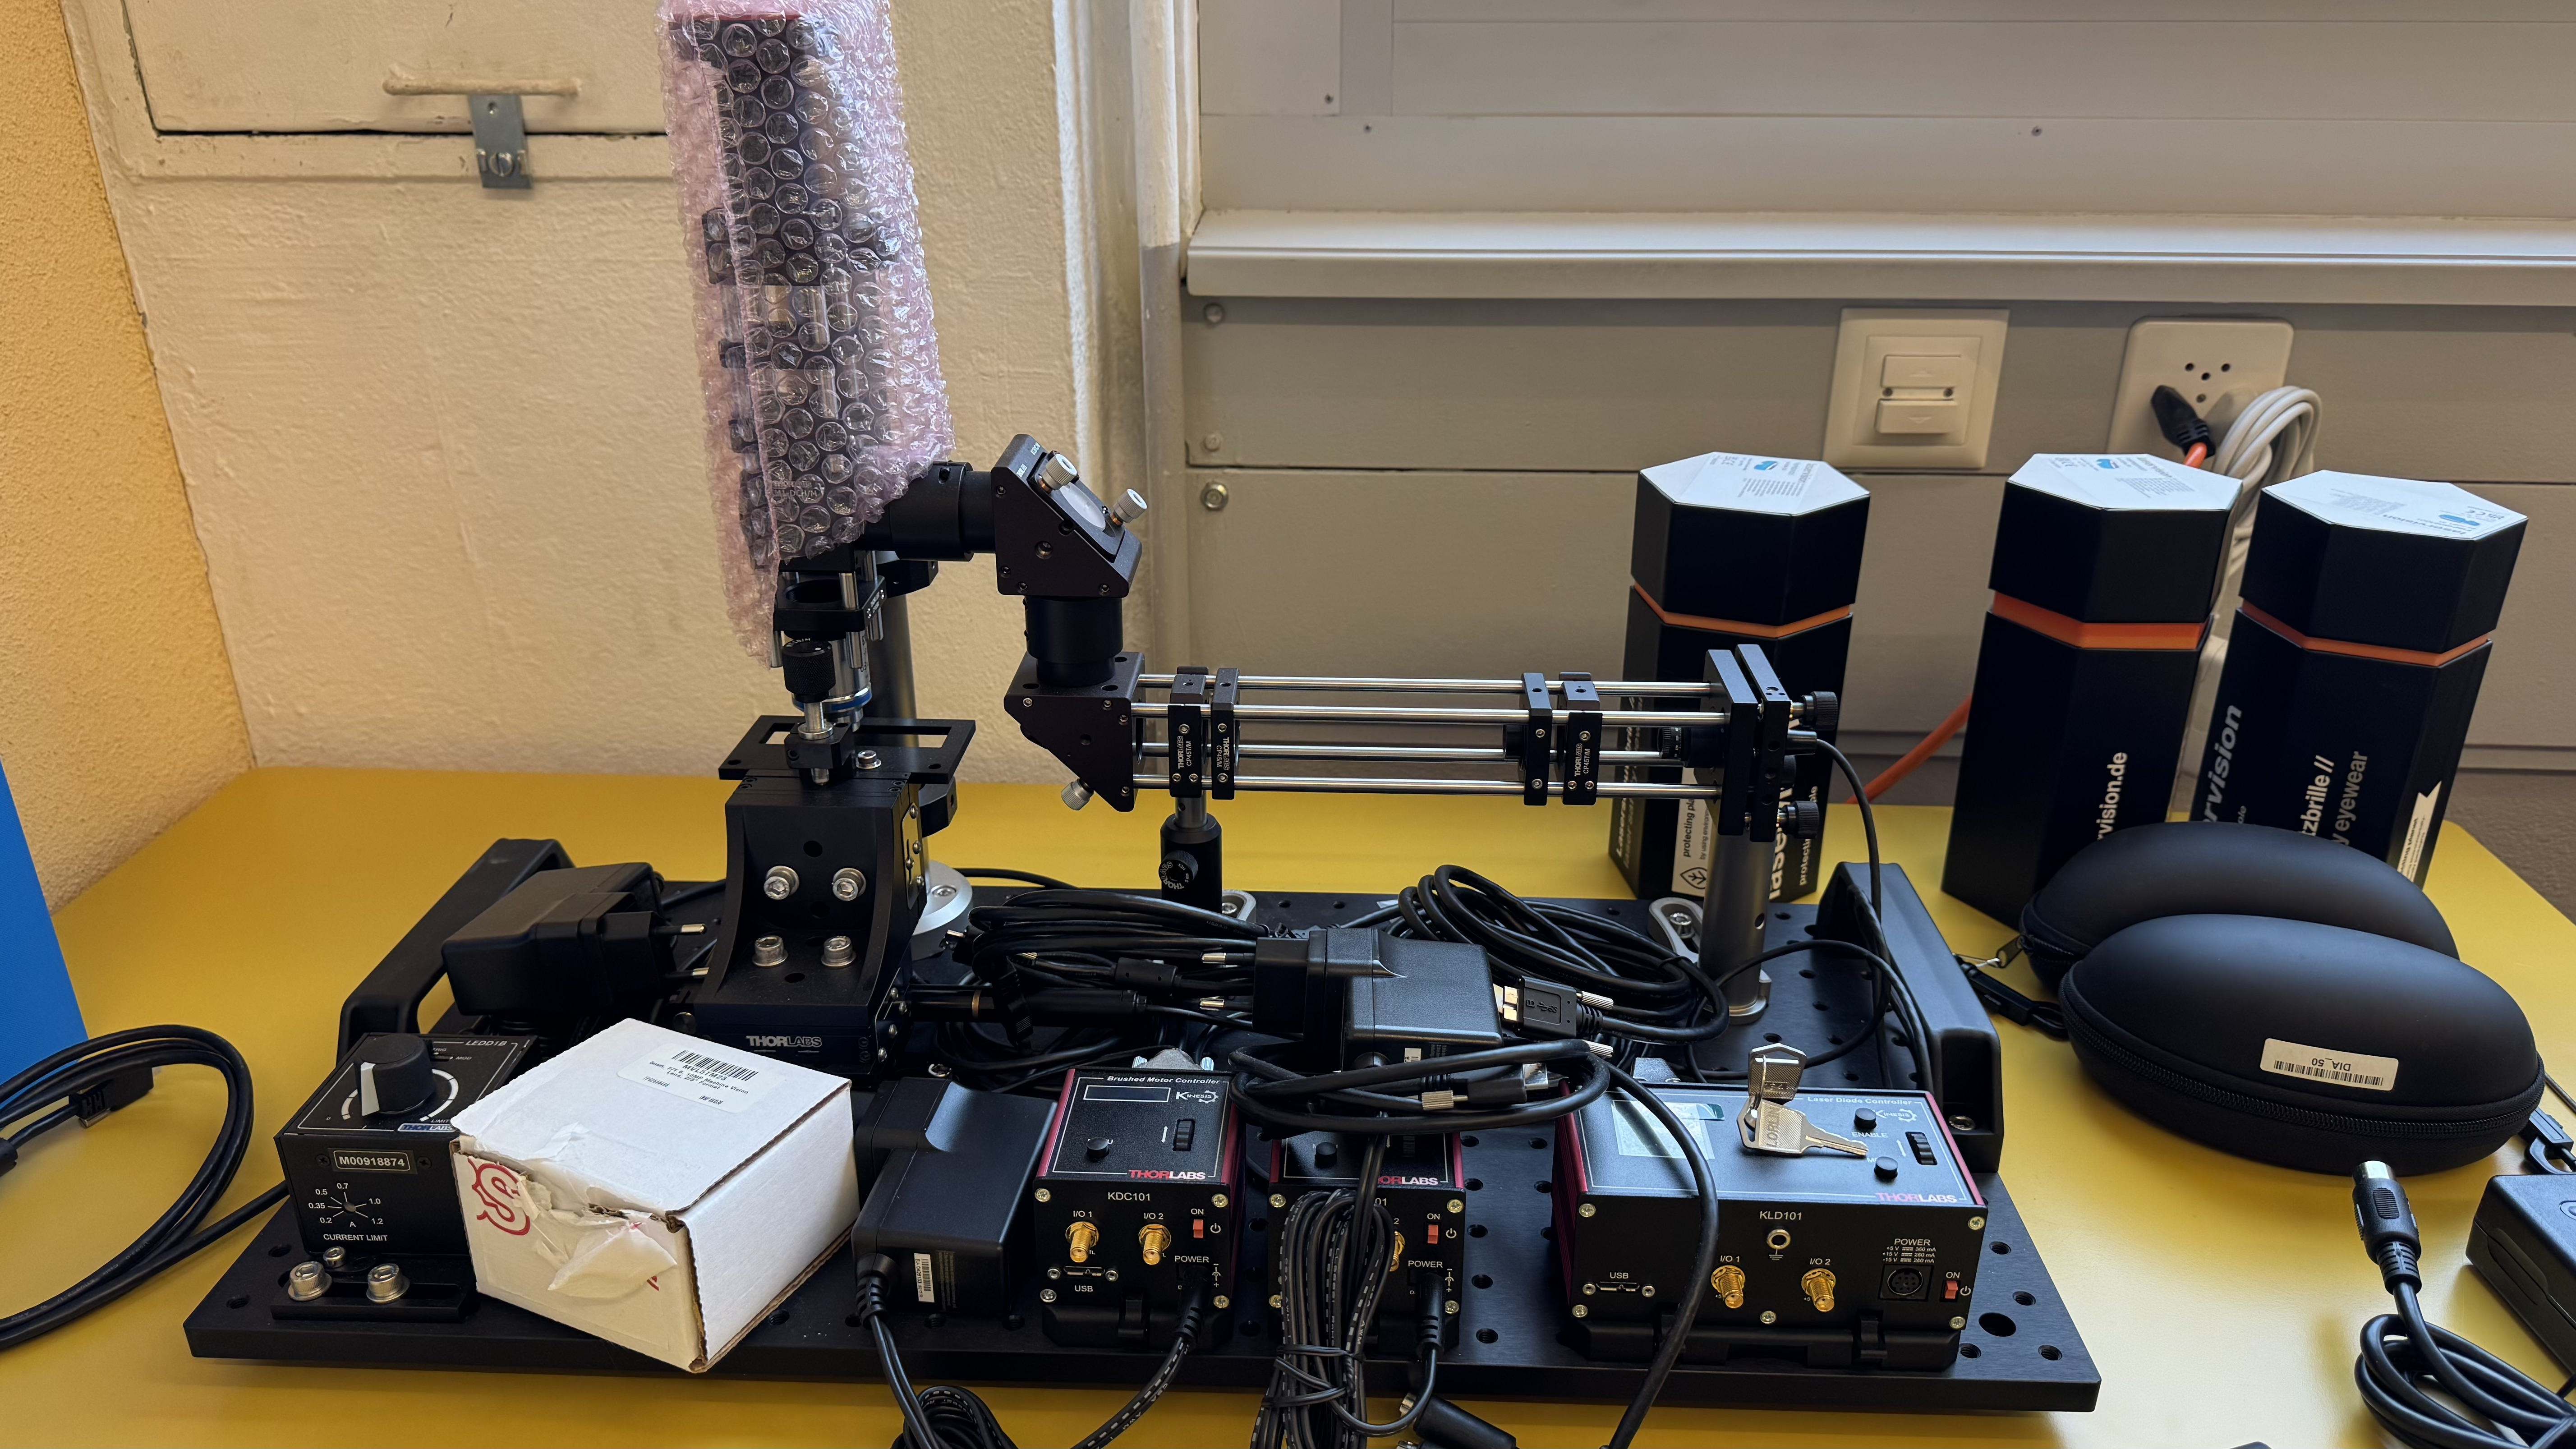
\includegraphics[width=0.7\textwidth]{assets/figures/Introduction/kit_vierge.jpeg}
    \end{center}
    \caption{Kit Portable Optical Tweezers de Thorlabs}
    \label{kit_vierge}
\end{figure}

Une représentation 3D du kit, accompagnée de légendes pour chaque composant, a été réalisé par mes soins. Ce modèle CAO permet une clareté et une compréhension plus rapide des différents éléments. Les différentes modélisations 3D des composants ont directement été pris du site Thorlab. Je me suis chargé de les rassembler dans un seul fichier CAO et de faire l'assemblage (voir Figure \ref{kit_CAO_vierge_annote}).

\begin{figure}[H]
    \begin{center}
        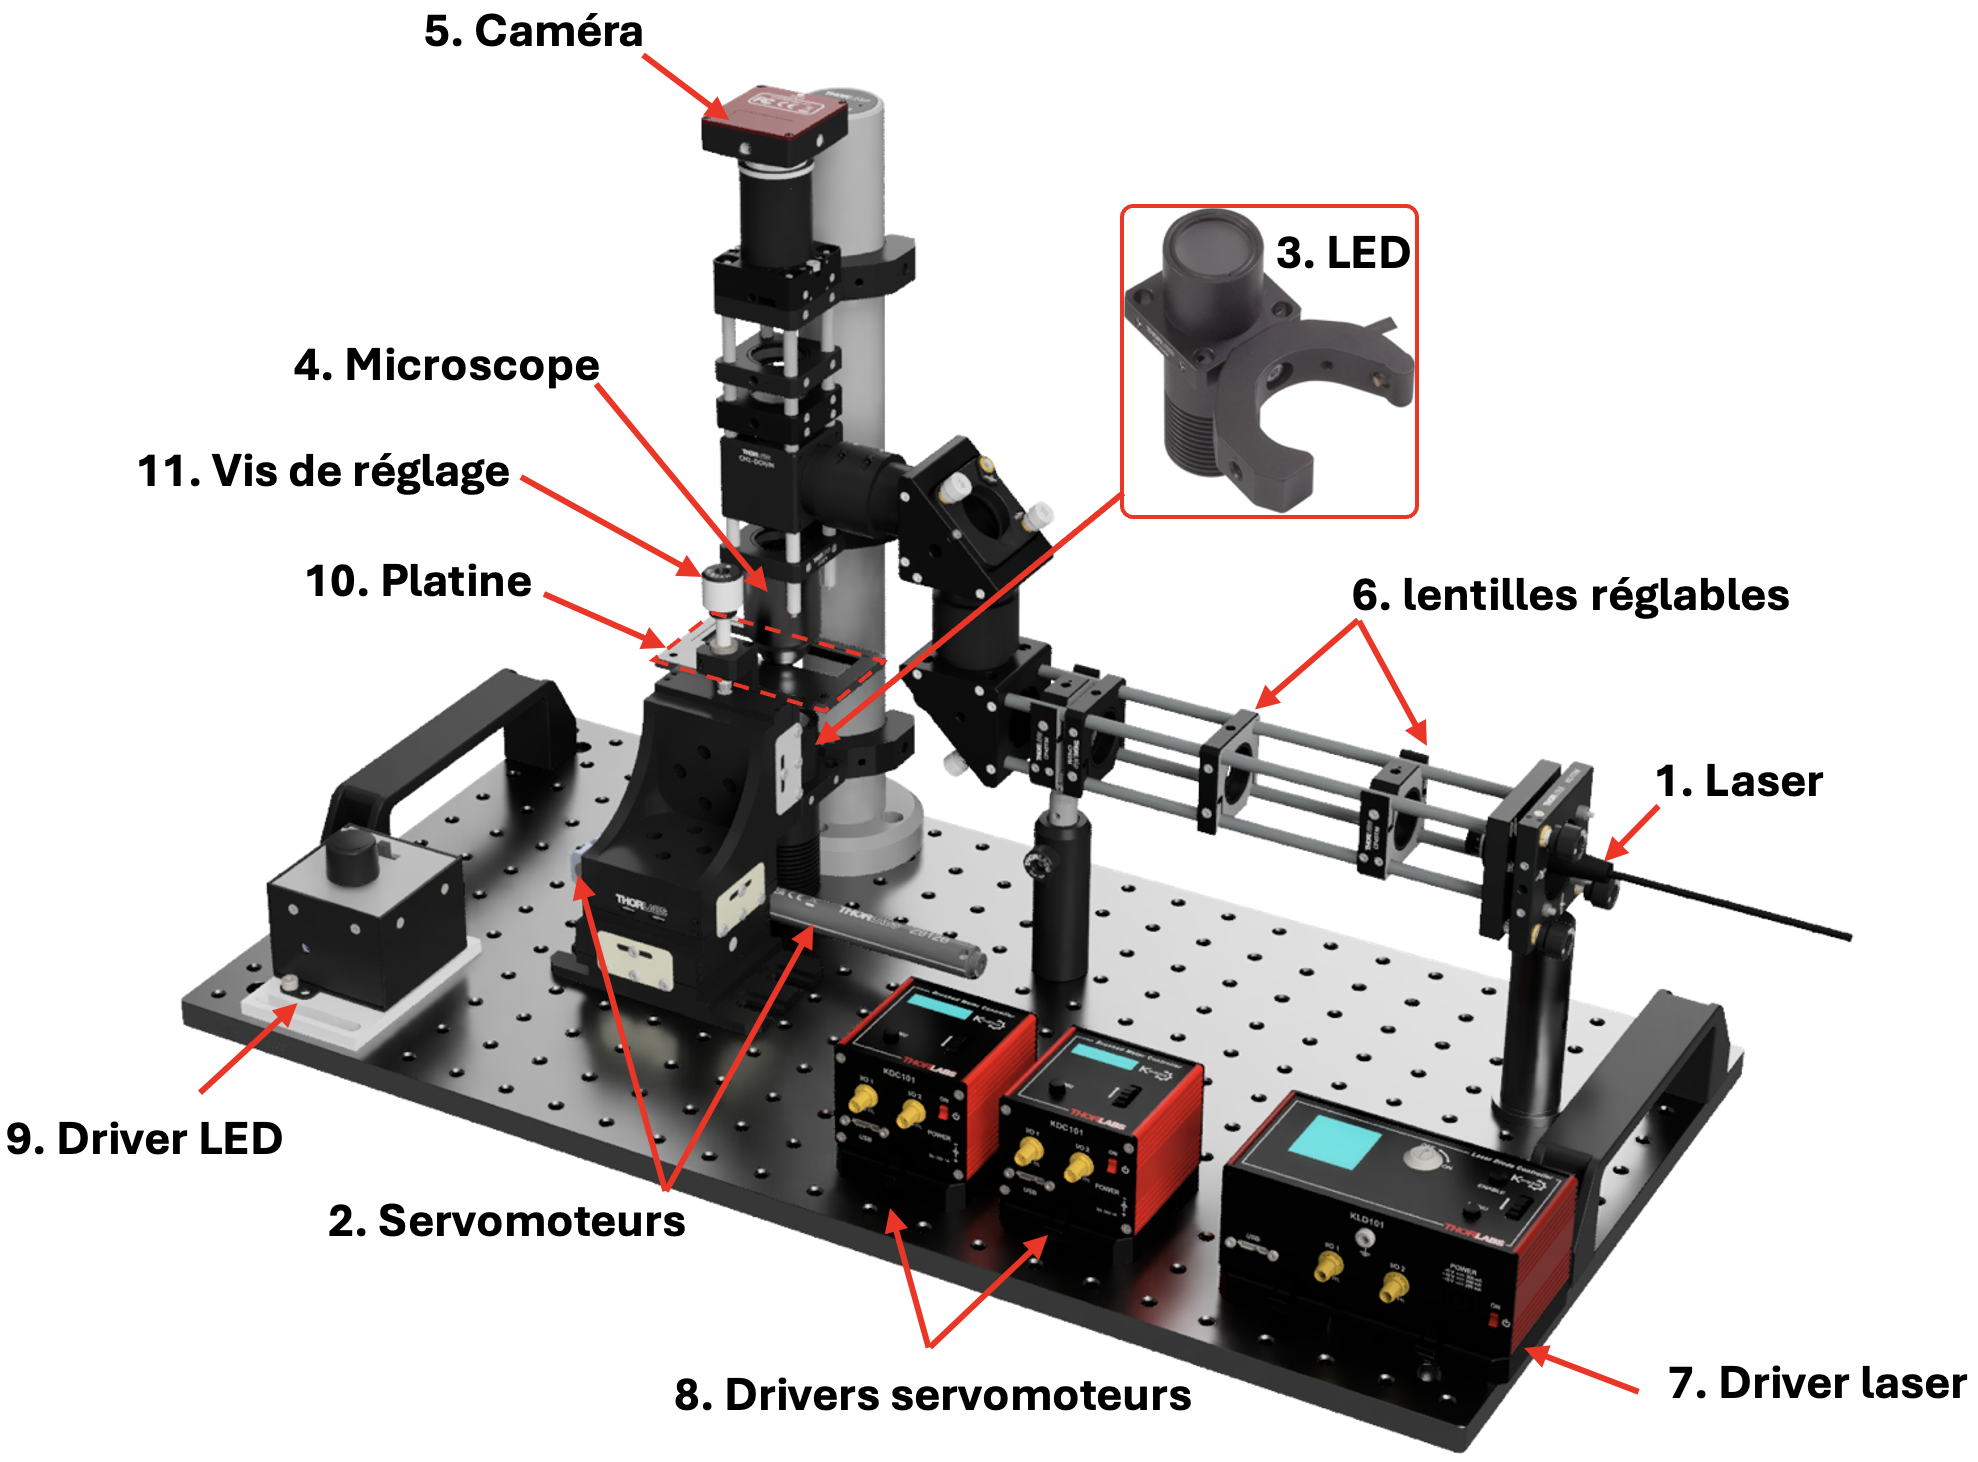
\includegraphics[width=0.7\textwidth]{assets/figures/Introduction/Kit_CAO_vierge_annote.png}
    \end{center}
    \caption{CAO du kit avec annotations des principaux composants}
    \label{kit_CAO_vierge_annote}
\end{figure}

\begin{enumerate}
    \item Laser d'une longueur d'onde 658 nm et de puissance maximum 40 mW.
    \item Les servomoteurs permettent de déplacer la platine en X Y.
    \item La LED permet un réglage manuel de l'éclairage.
    \item Microscope équipé d'un objectif avec un grossissement de $63\times$ et une ouverture numérique de 0,8.
    \item
\end{enumerate}

\section{Objectifs}

Les différents objectifs de ce travail de bachelor sont listés ci-dessous :
\begin{enumerate}
    \item Mettre en service le kit : câblage, calibration du laser
    \item Conception de protection contre le laser afin d'apporter plus de sécurité lors de l'utilisation du kit
    \item Élaboration d'une notice de laboratoire compacte pour utiliser simplement le kit
    \item Effectuer des tests de déplacements de microbilles dans différents milieux, de différentes viscosités, dans différents types de réservoirs ainsi que de multiples canaux.
    \item Analyses expérimentales des forces de déplacement en fonction de la viscosité des fluides
\end{enumerate}

\subsection{Mise en service du kit}

La première partie consiste à mettre en service le kit. Il faut alimenter les différents drivers qui contrôlent les moteurs, la LED ainsi que le driver pour le laser. Viens ensuite la procédure de calibration du laser, ainsi que l'installation des logiciels permettant de contrôler, d'une part les drivers des moteurs, et d'autre part le driver du laser.
\subsection{Protections contre le laser}
La deuxième partie porte sur la conception des protections contre le laser. Deux parties du kit ont besoin d'avoir une protection totale afin d'éviter toutes reflexions nocives du laser dans les yeux de l'utilisateur. La première protection à réaliser est située au début du laser et va devoir entouré toute la cage oû le laser passe (voir Figure \ref{protection_laser_début}). L'encadré en \textcolor{red}{rouge} représente l'endroit où va devoir être imaginer la protection.

\begin{figure}[H]
    \begin{center}
        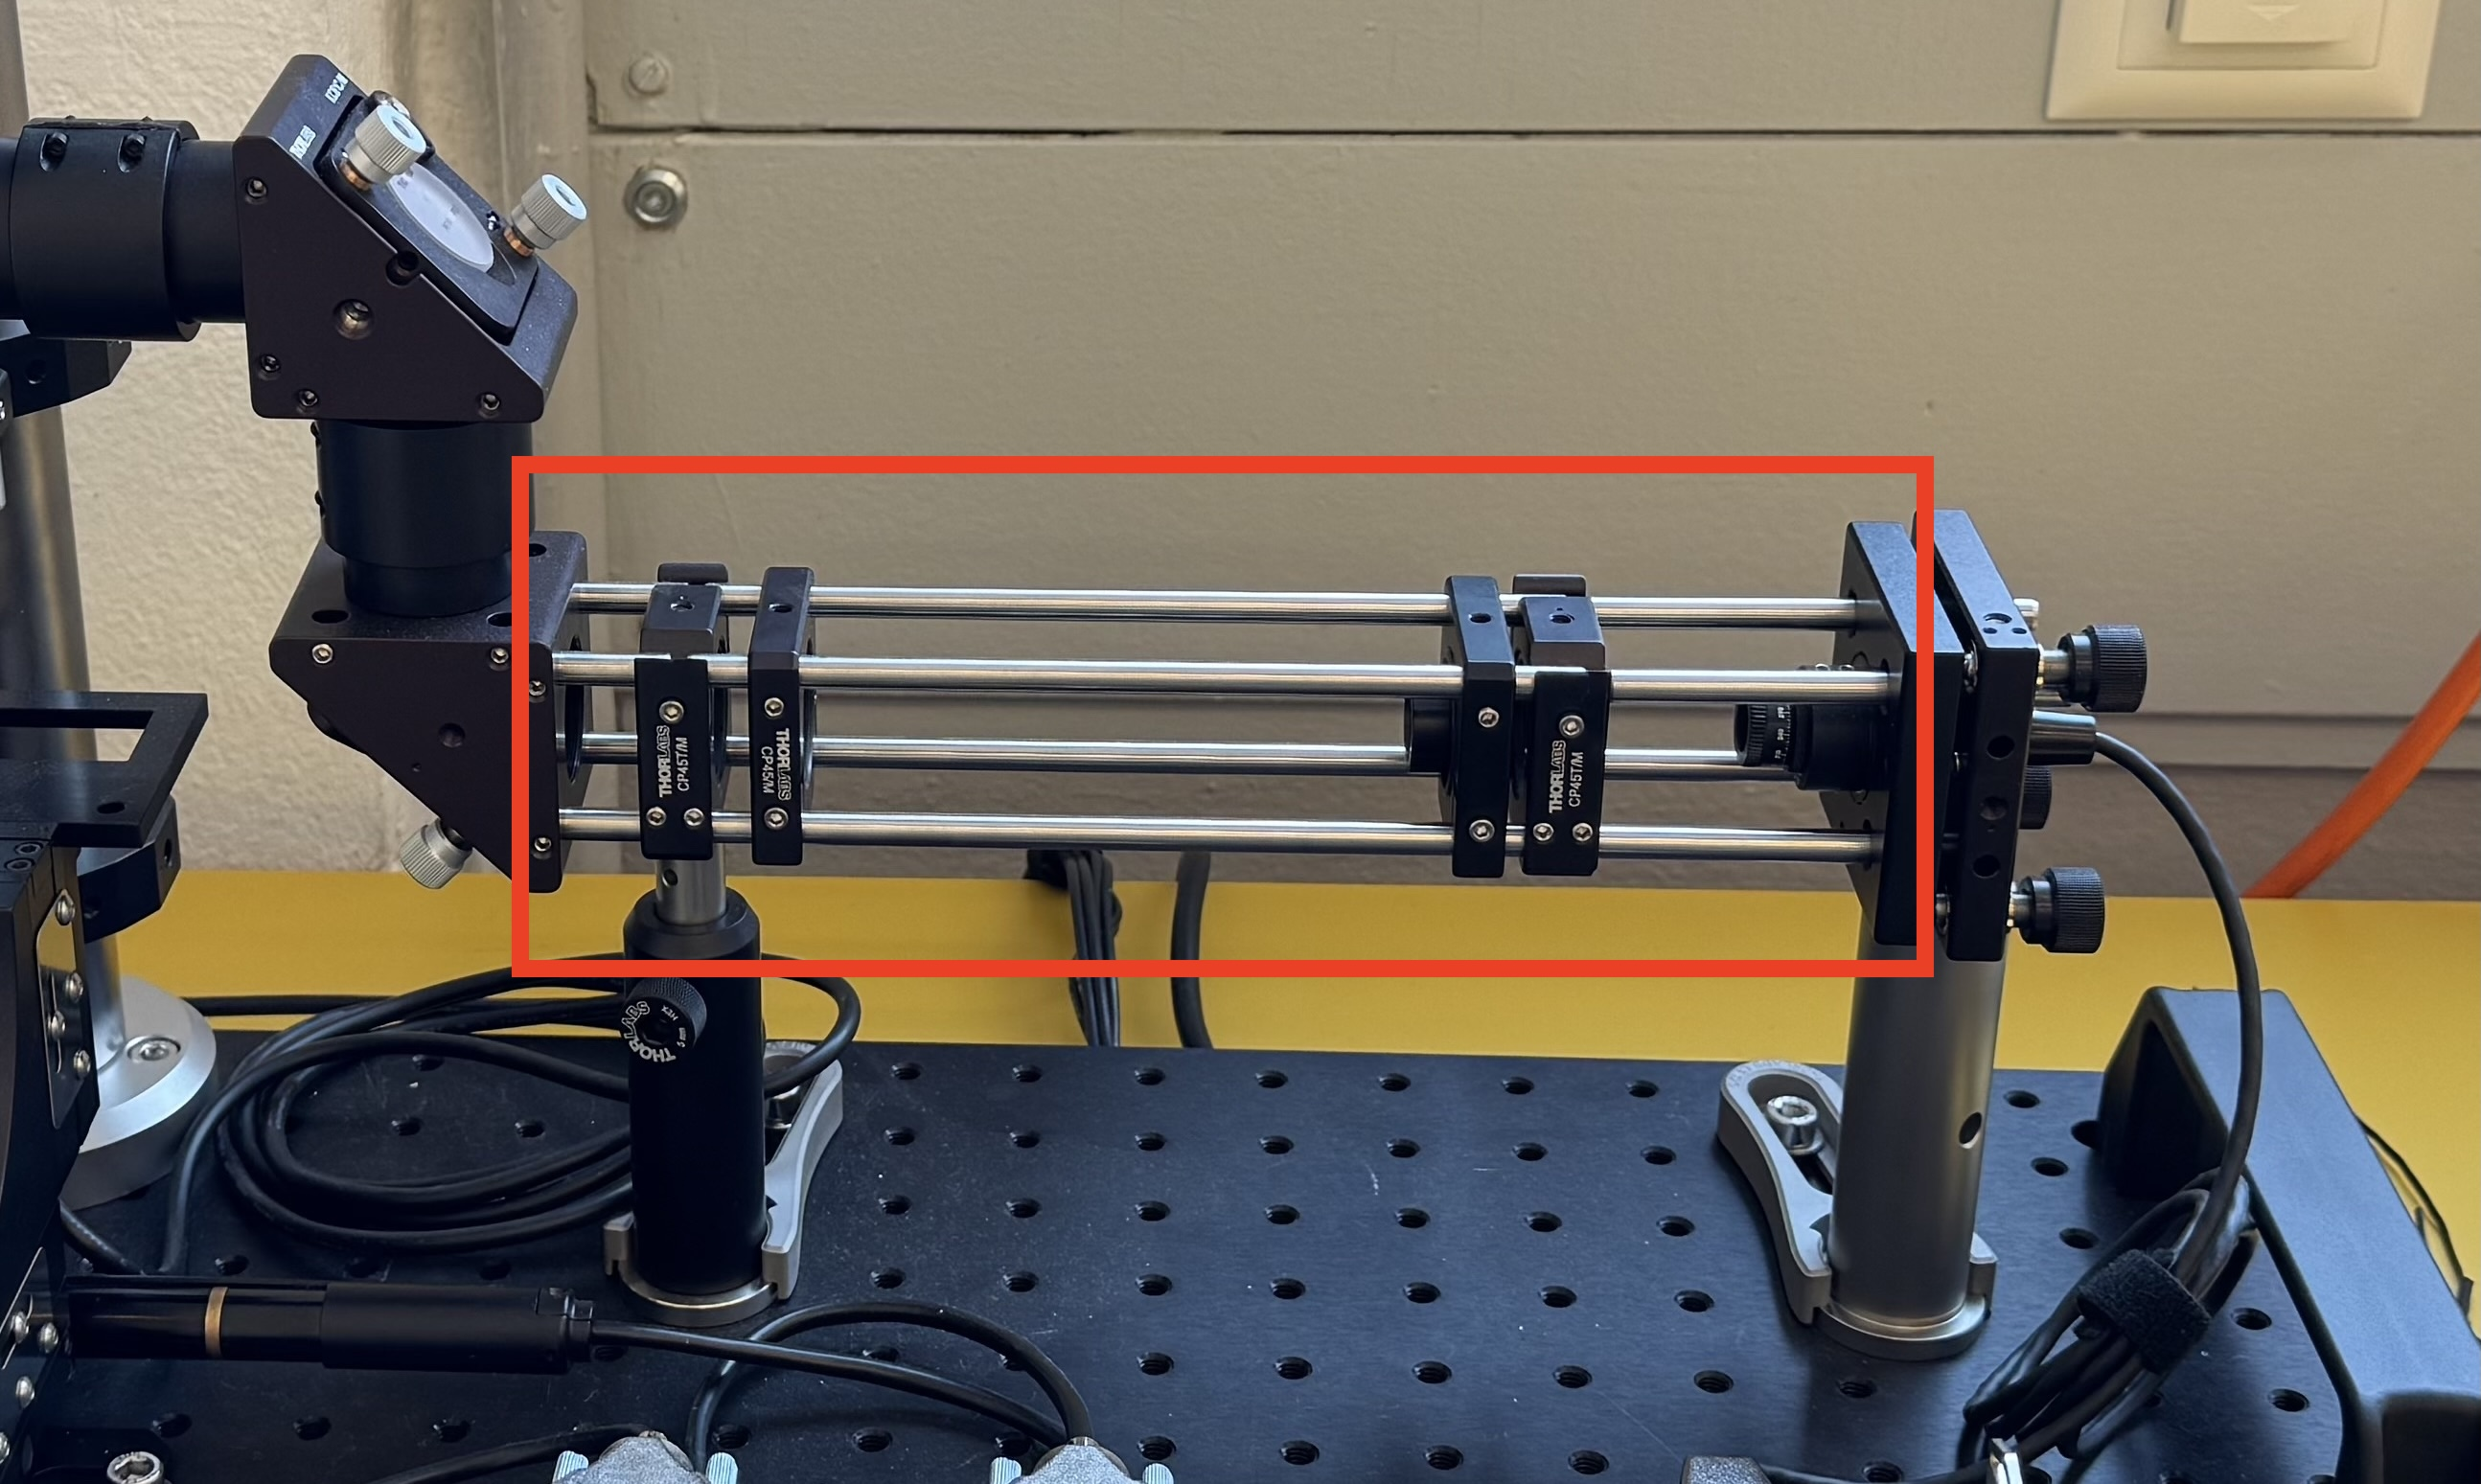
\includegraphics[width=0.5\textwidth]{assets/figures/Introduction/protection_debut_laser.jpeg}
    \end{center}
    \caption{Première protection contre le laser située vers le laser}
    \label{protection_laser_début}
\end{figure}

Une deuxième protection va être faite vers le microscope, car également à cet endroit, le laser devient visible à l'oeil nu et il y'a un grand risque de se blesser. L'encadré en \textcolor{blue}{bleu} représente l'endroit où va devoir être imaginer la protection. Voir la Figure \ref{protection_laser_fin}.

\begin{figure}[H]
    \begin{center}
        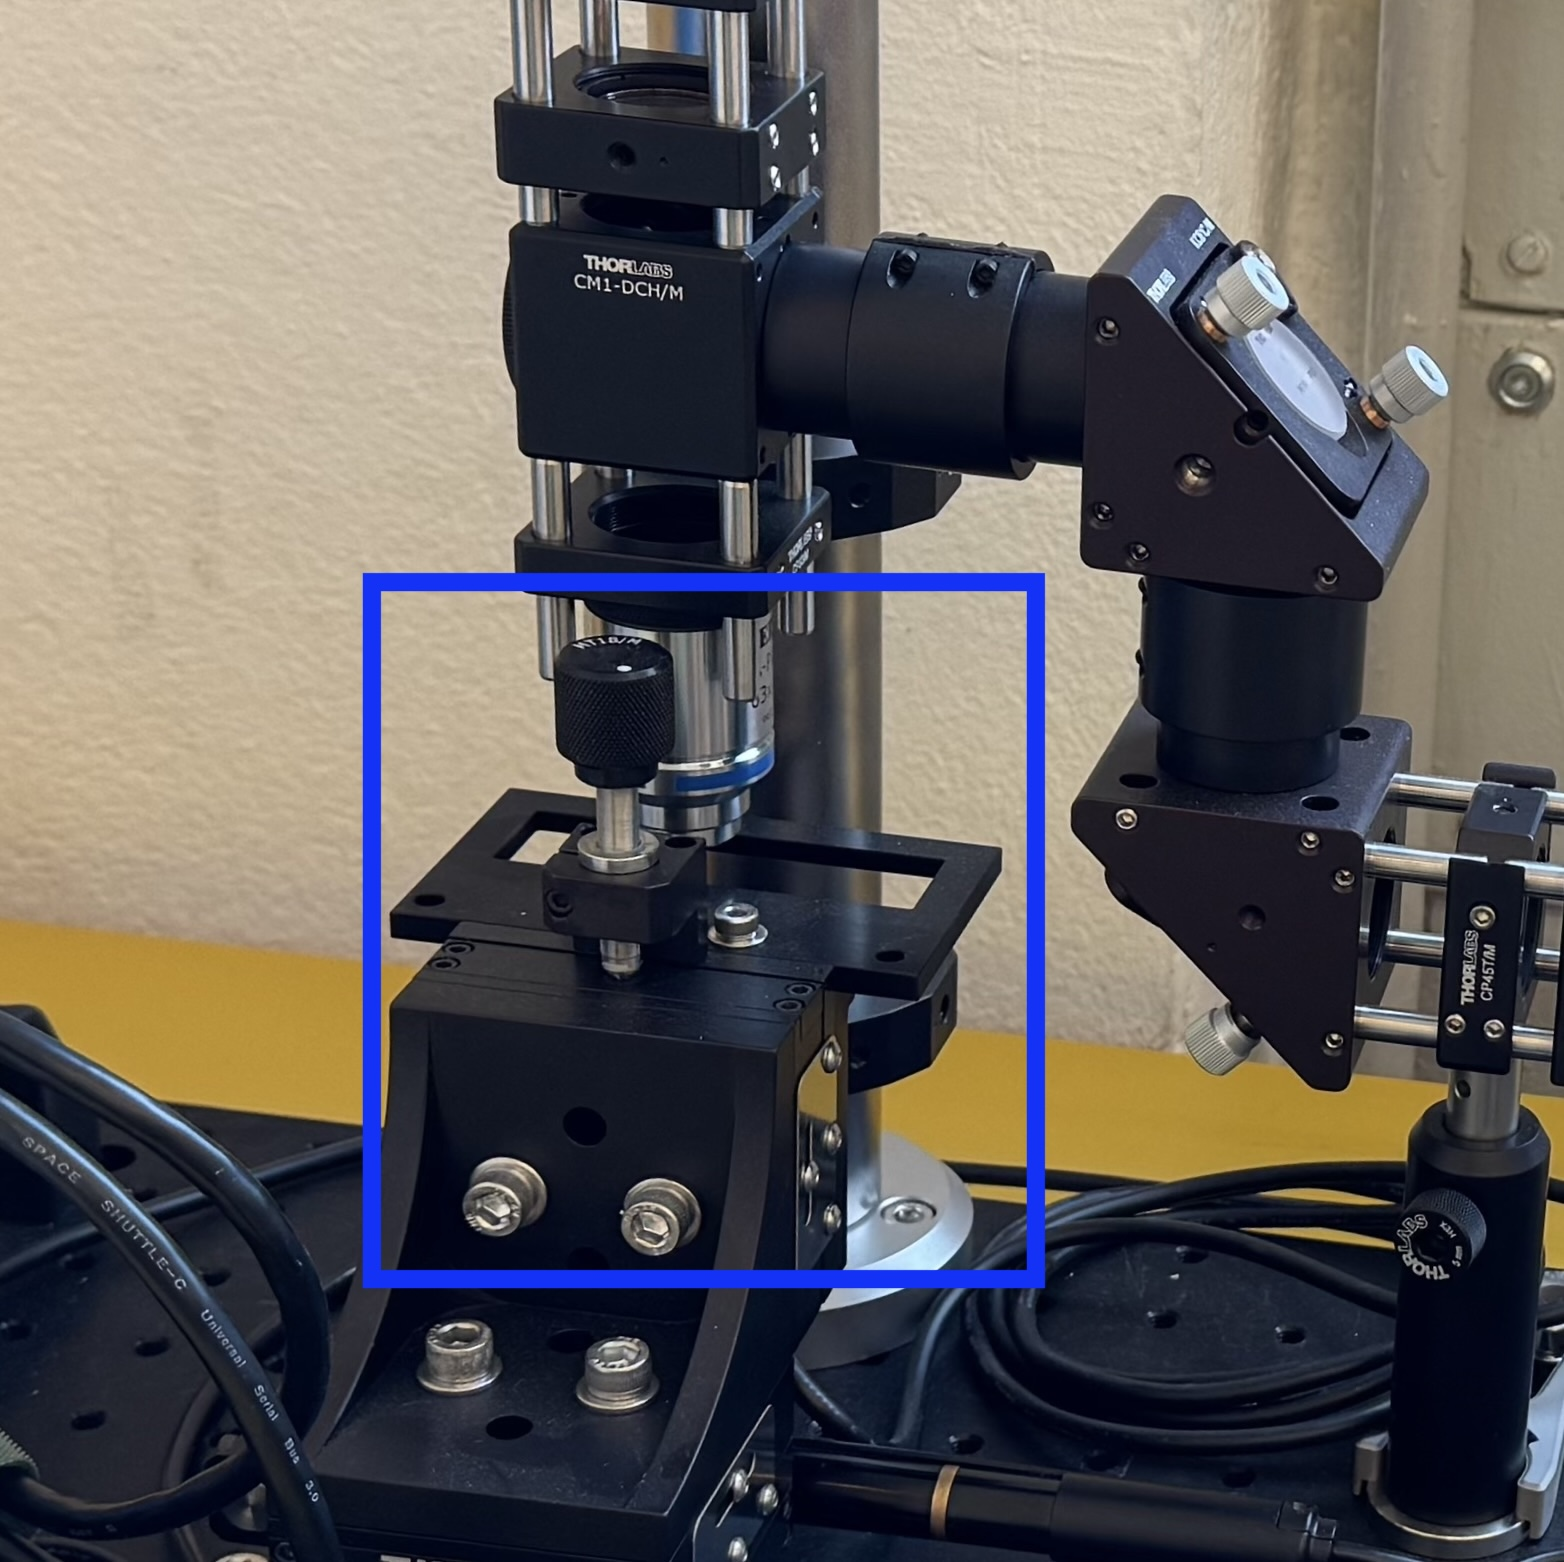
\includegraphics[width=0.5\textwidth]{assets/figures/Introduction/protection_fin_laser.jpeg}
    \end{center}
    \caption{Deuxième protection contre le laser située vers le microscope}
    \label{protection_laser_fin}
\end{figure}

\subsection{Notice de laboratoire}

Un des objectifs de ce TB, consite également à créer une notice de laboratoire pour un cours d'étudiants de la filière système industriels. Cette notice devra être simple à comprendre, compacte et comprendra des manipulations avec différents liquides, ainsi que des mesures pratiques.

%%if
\section{Citations et bibliographie}
Citer vos sources est essentiel. Avec \texttt{biblatex} vous pouvez facilement citer des articles, des livres ou des sites internet. Toutes les citations dans le texte seront automatiquement regroupées en fin de document dans la section \guillemotleft Bibliographie\guillemotright. Par exemple, citons un article d'Einstein \cite{einstein} ou le livre de Dirac \cite{dirac}.

Parfois il peut être utile d'utiliser un gestionnaire de bibliographie. La communauté académique recommande l'outil \href{https://www.zotero.org/}{Zotero} qui permet de gérer une bibliothèque numérique d'ouvrages et de références numériques. Il permet également de générer une bibliographie compatible avec \LaTeX.

Notez qu'il est très facile d'obtenir l'extrait \texttt{bibtex} depuis des journaux. Sélectionnez \emph{export/citation}. Si vous le pouvez choisissez \texttt{bibtex}. Dans le cas d'un format \texttt{.ris}, utilisez un convertisseur en ligne comme \href{http://www.bruot.org/ris2bib/}{ris2bib}.

\section{Adapter votre modèle}
Ce document n'est qu'un modèle ayant pour but de revoir les quelques avantages de \LaTeX~ et les fonctionnalités qui pourraient vous être utiles pour rédiger un rapport académique. N'hésitez pas à supprimer les parties inutiles et à adapter ce modèle à vos besoins.
%%fi